%%%%%%%%%%%%%%%%%%%%%%%%%%%%%%%%%%%%%%%%%%%%
\section{Selection of Raster Fields [TBD]\label{sec:RasterField}}

In this section, we describe the preparation of target stars in order to carry out the raster scan during the engineering observations. The stars should be sufficiently bright and the number density should be matched to the number of fibers in the PFS FoV. The most plausible candidate is an open cluster. Here, we describe the selection of the raster field and the possible target stars. 

\subsection{Open Clusters as the Raster Targets}
Open clusters in the Galaxy are possible target of stars for the raster observations. The open clusters are selected from DAML02 catalogue (Dias et al. 2002, A\&A, 389, 871), which includes information on fundamental parameters (distance, apparent diameter, proper motion, age, reddening, metallicity, and so on) of $\sim2000$ open clusters. 

Figure \ref{fig:RasterFieldMap1} and Figure \ref{fig:RasterFieldMap2} show the spatial distribution of the open clusters with the apparent diameter ($d$ [deg.]) of $>30$. There exist $\sim130$, $\sim50$, $\sim30$ open clusters with the apparent diameter of $30<d<60$, $60<d<120$, and $d>120$, respectively. The typical number of member stars is $\sim1000$. 

\subsection{Field Stars}
As Figure \ref{fig:RasterFieldMap1} and Figure \ref{fig:RasterFieldMap2} show, the spatial location of the available open clusters with sufficient apparent diameter for the PFS FoV is very limited. We thus consider the possibility of using normal field stars as raster scan targets in this subsection. In Figure \ref{fig:RasterFieldMap1} and Figure \ref{fig:RasterFieldMap2}, the density map of stars with $f<16.0$ mag. selected from the UCAC4 catalogue (Zacharias et al. 2013, AJ, 145, 44), which contains 113 million stars down to $R\sim16$ mag for which the positions determined with the accuracy of $<100$ mas. Although the number of available stars in one PFS FoV is limited in the high galactic latitude ($b$), there exist sufficient available stars of $<16$ mag in $b<60$ deg.

\subsection{Detailed Procedure of Raster Scan}
TBW

\subsection{List of Candidate Raster Fields}
TBW

\begin{figure}[!ht]
\begin{center}
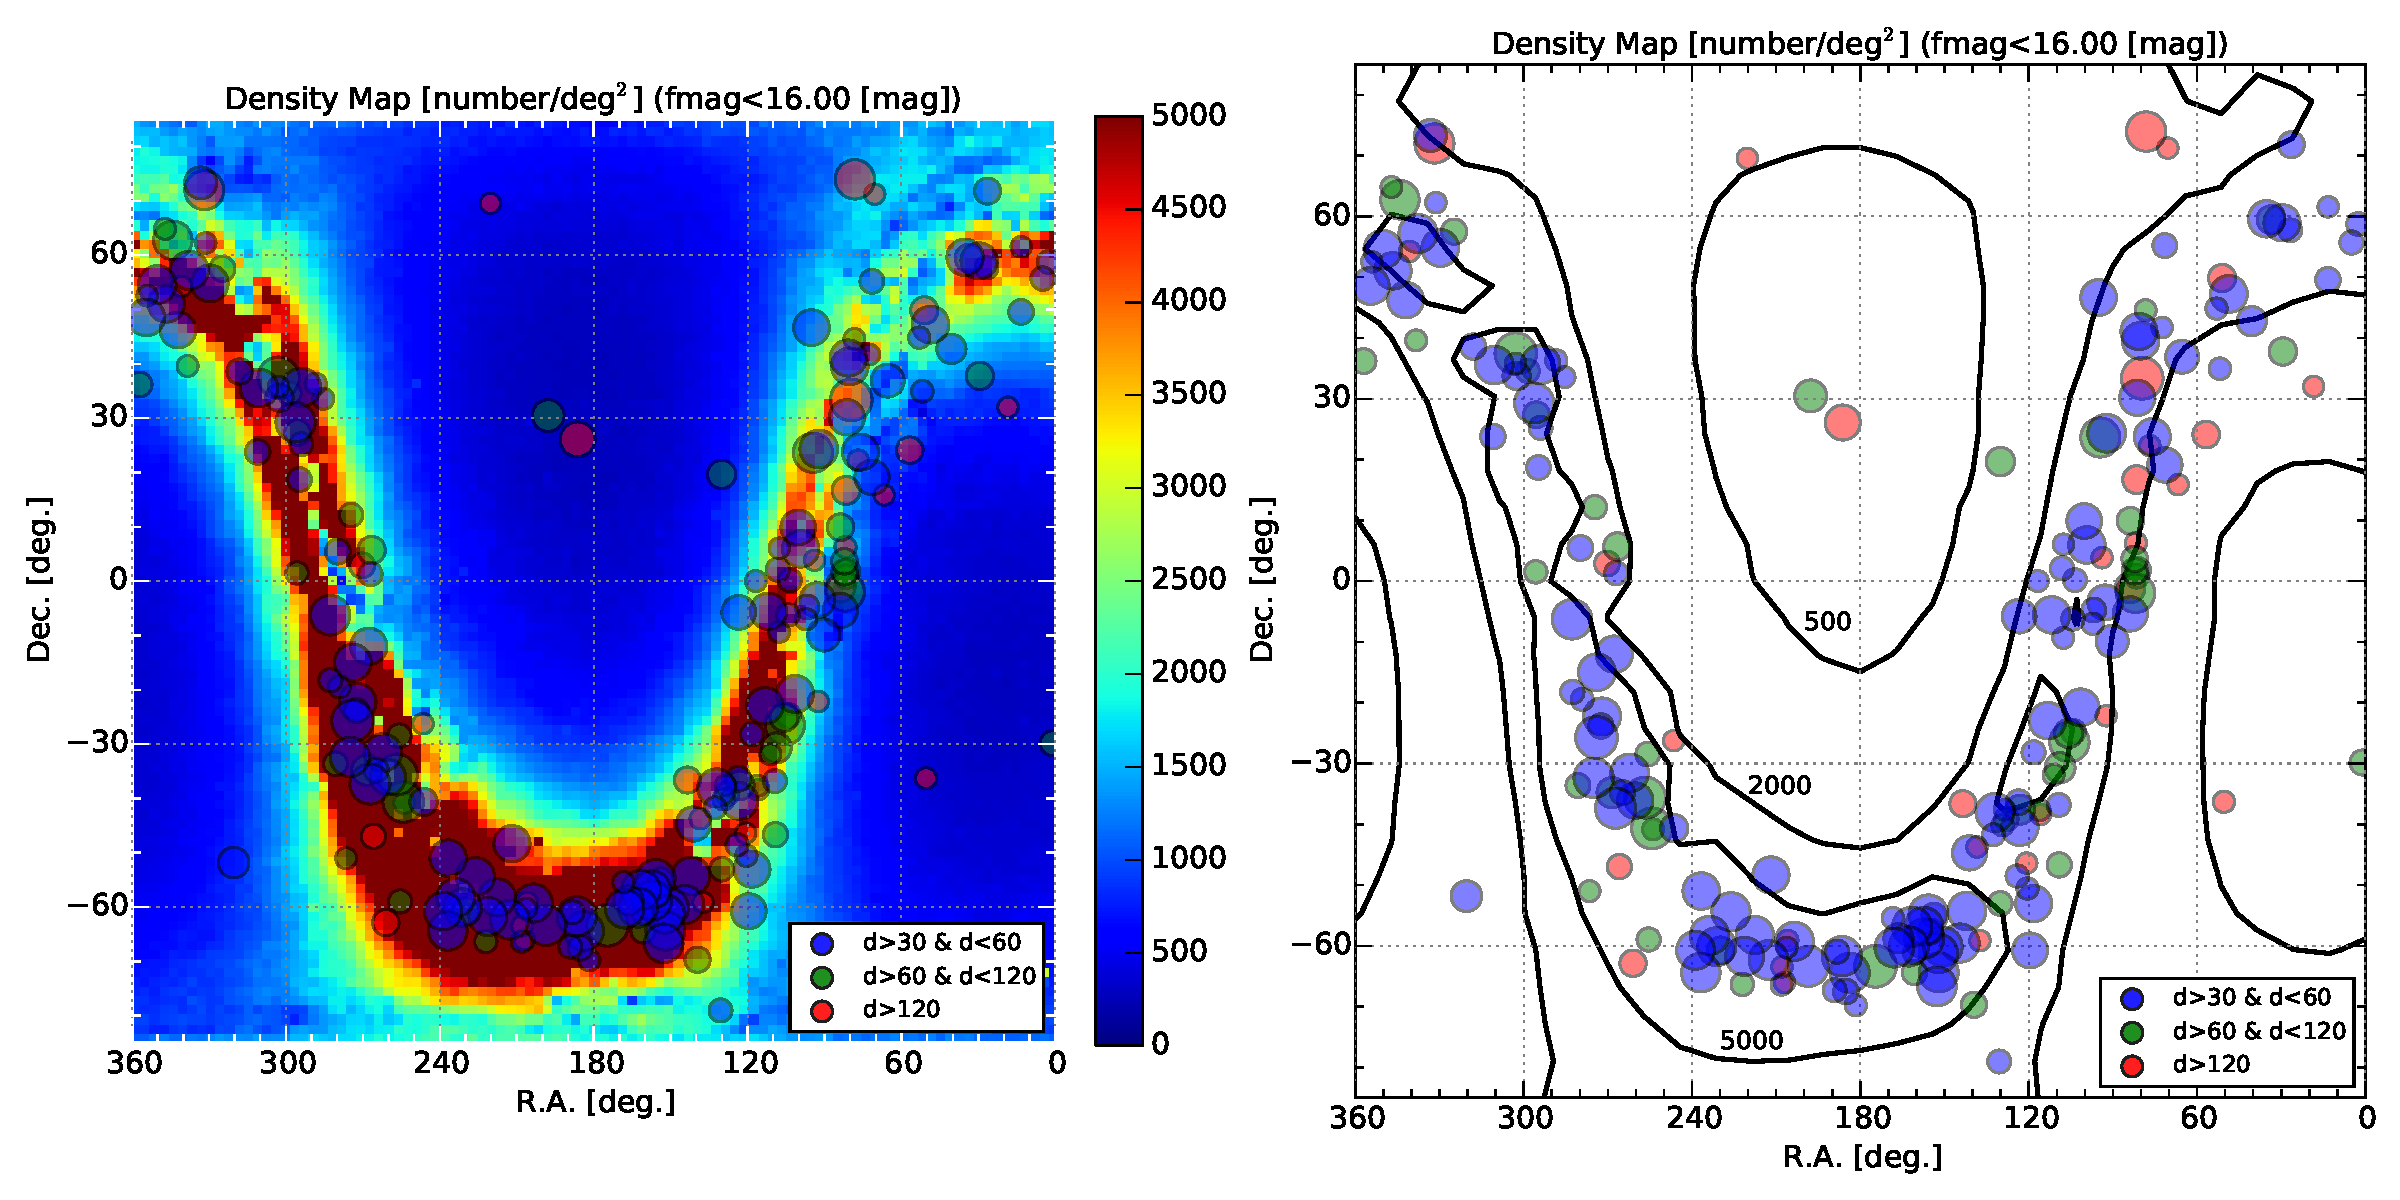
\includegraphics[width=150mm]{map_f16mag_cont_openclusters_combined_20151208.pdf}
\end{center}
\caption{Stellar density with objects $f<16.0$ mag taken from UCAC4 catalog in color map (left) and contour (right). The spatial distribution of open clusters with the apparent diameter ($d$ [deg.]) of $d>30$. from DAML02 catalogue is also plotted in both panels. Open clusters with $30<d<60$, $60<d<120$, and $d>120$ are shown by \textit{blue}, \textit{green}, and \textit{red circles}, respectively. The size of symbols represents the number of member stars.
}
\label{fig:RasterFieldMap1}
\end{figure}

\begin{figure}[!ht]
\begin{center}
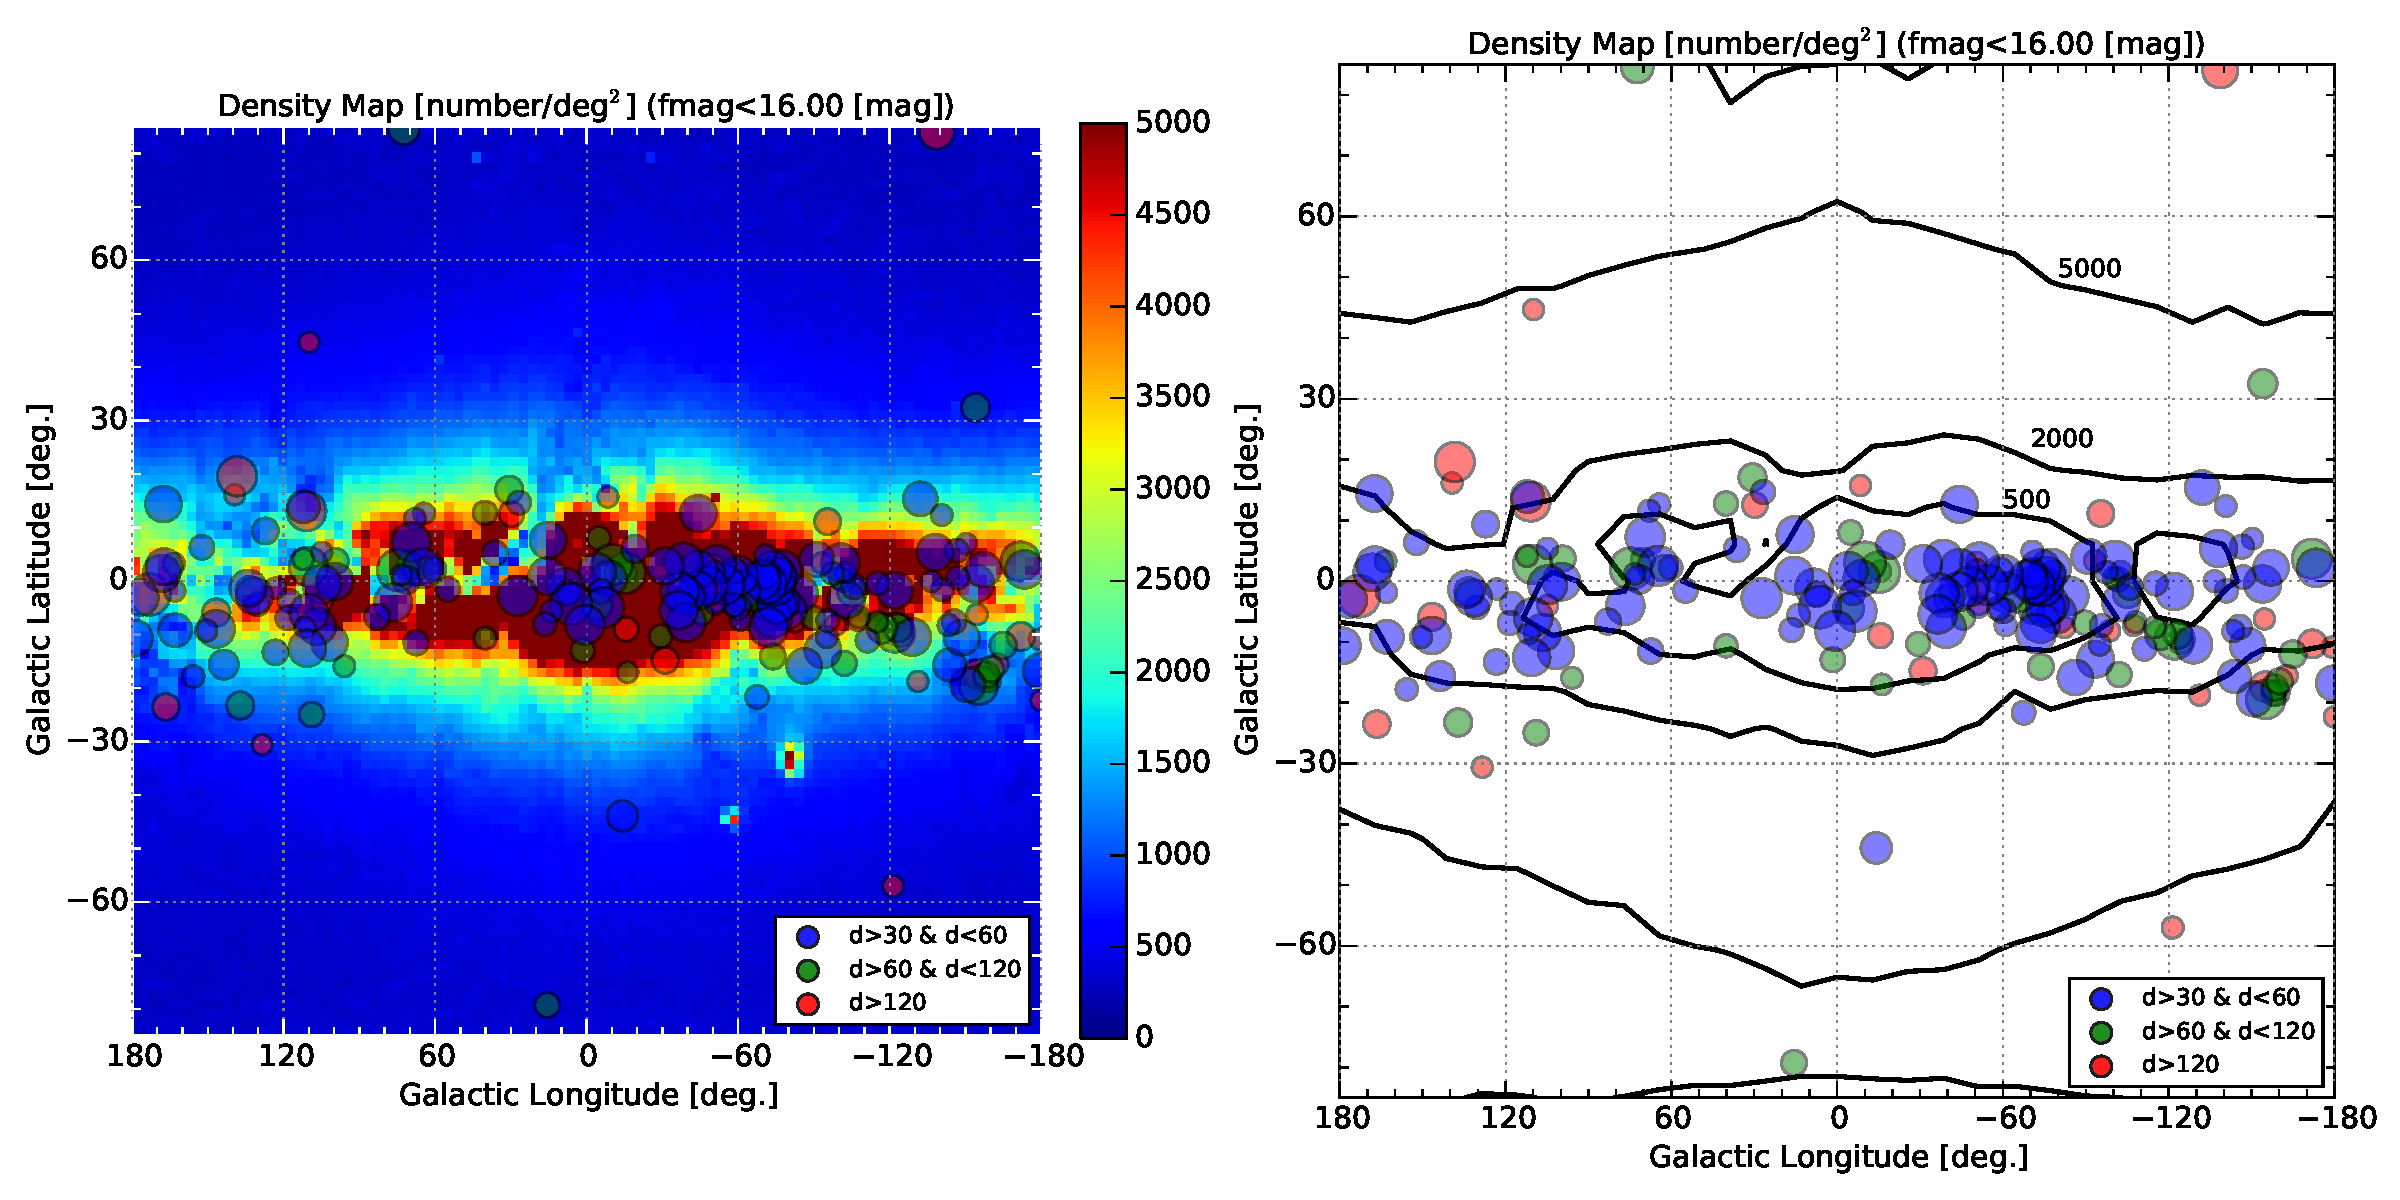
\includegraphics[width=150mm]{map_f16mag_cont_openclusters_gc_combined_20151208.pdf}
\end{center}
\caption{Similar to Figure \ref{fig:RasterFieldMap1}, but on the Galactic longitude and latitude.
}
\label{fig:RasterFieldMap2}
\end{figure}

\begin{figure}[!ht]
\begin{center}
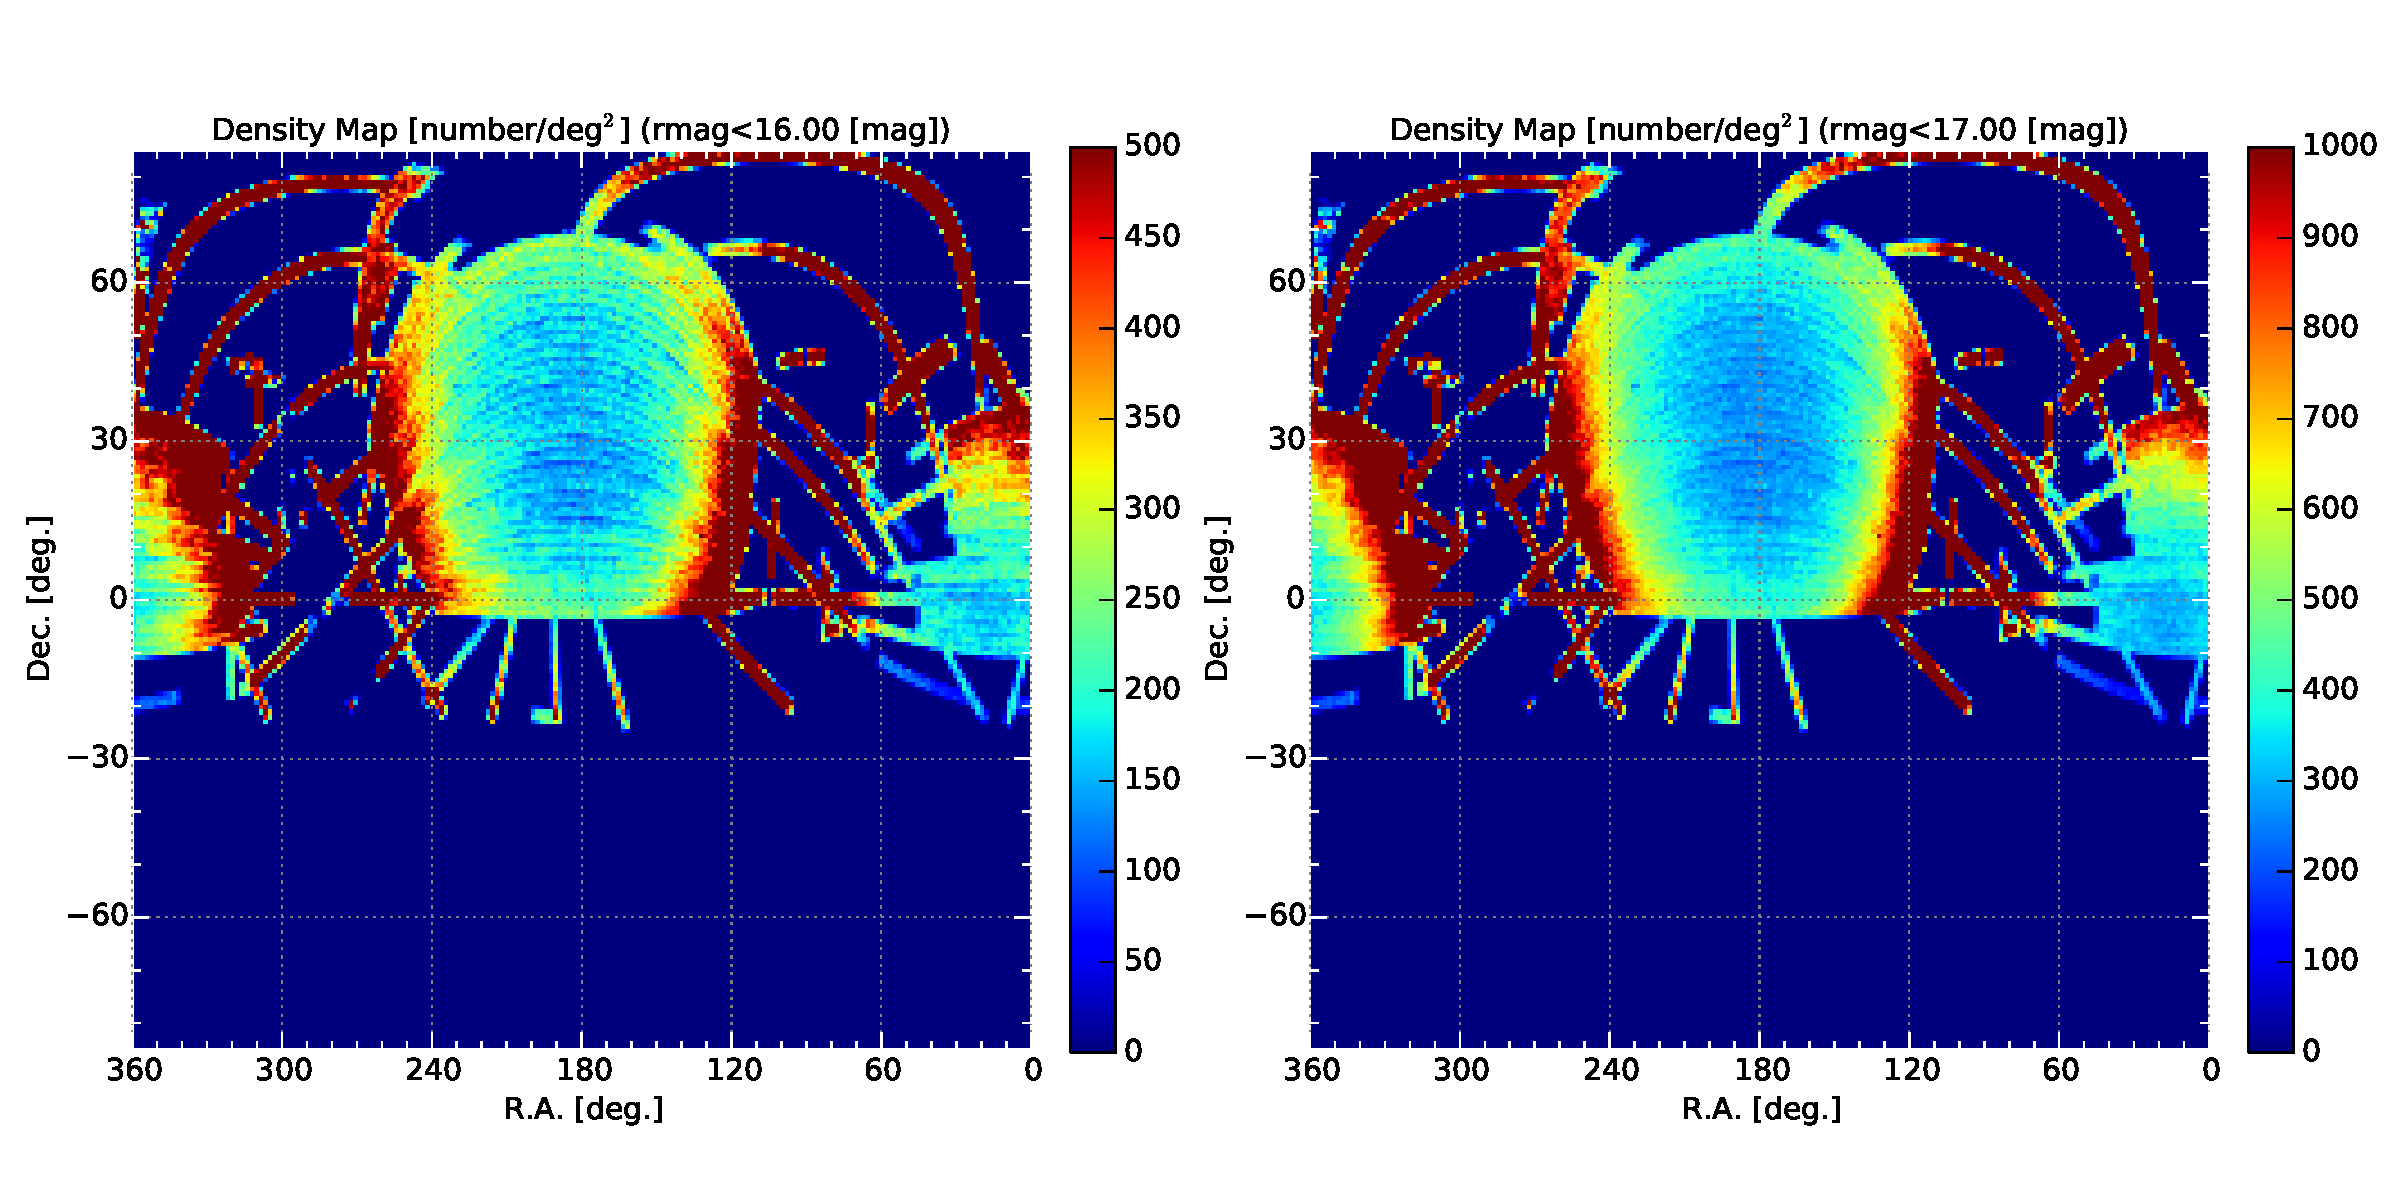
\includegraphics[width=150mm]{map_sdss_r16-17_colm_combined_20151208.pdf}
\end{center}
\caption{Stellar density with objects $r<16.0$ mag (left) and $r<17.0$ mag taken from SDSS DR12 catalog in color map. 
}
\label{fig:RasterFieldMapSDSS1}
\end{figure}

\begin{figure}[!ht]
\begin{center}
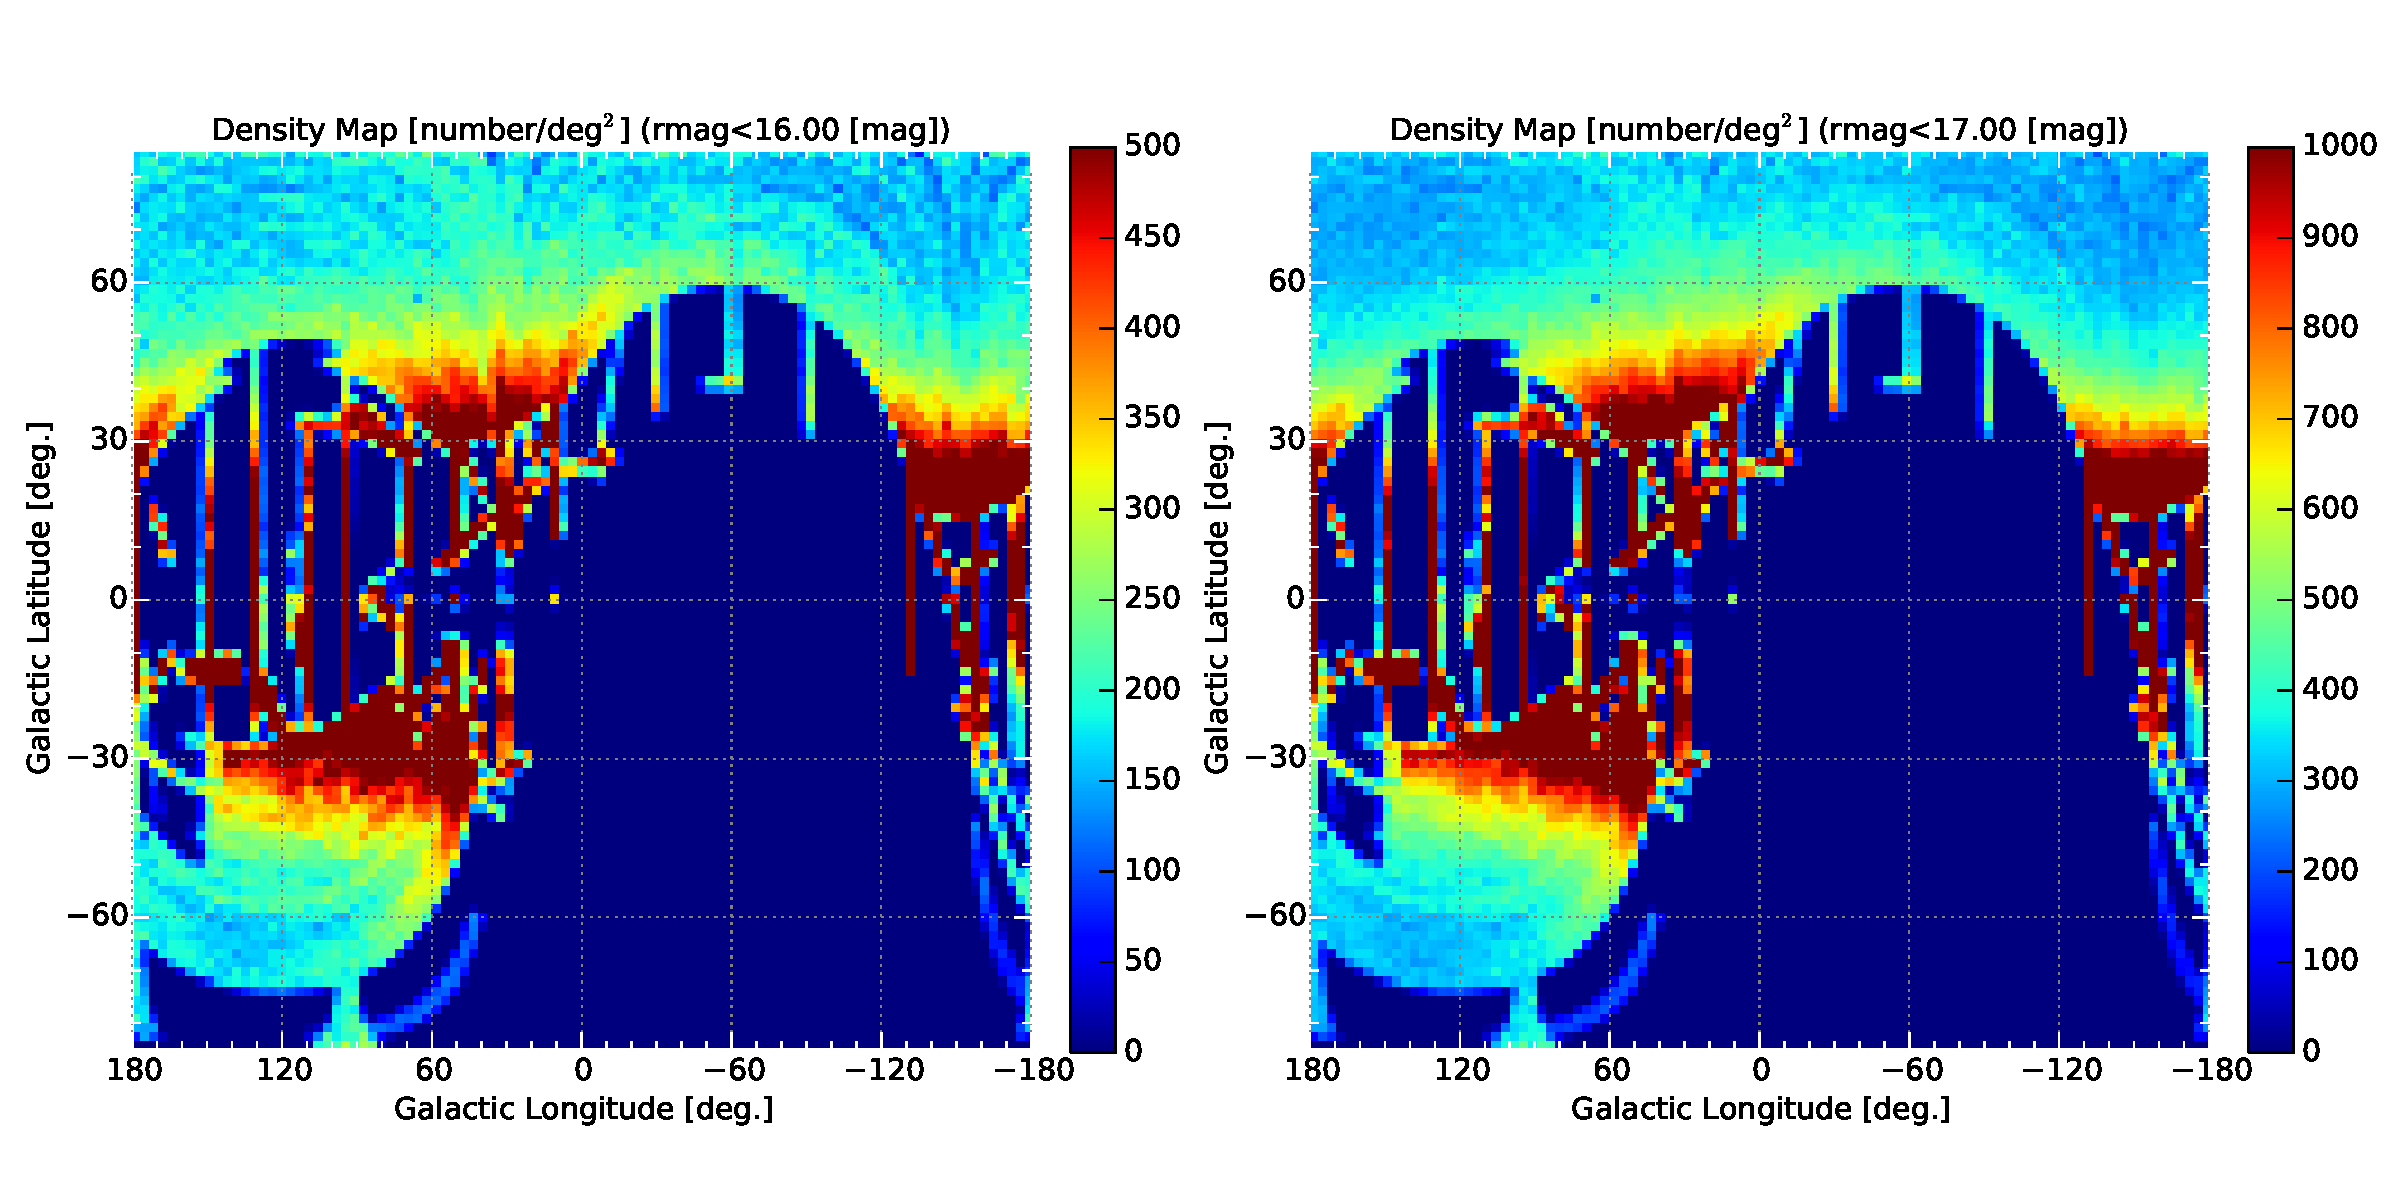
\includegraphics[width=150mm]{map_sdss_r16-17_colm_gc_combined_20151208.pdf}
\end{center}
\caption{Similar to Figure \ref{fig:RasterFieldMapSDSS1}, but on the Galactic longitude and latitude.
}
\label{fig:RasterFieldMapSDSS2}
\end{figure}
